\chapter{The Definition of a Graph}
\label{chapter:graph-theory-basics}
In this chapter we start a very important topic in discrete mathematics, which
became even more important with the rise of computers, we start the discussion
of graph theory. Graphs are used in mathematics and computer science to describe
networks, maps, and dependencies of objects.

\begin{definition}
  A \emph{graph} $G$ is a pair $(V, E)$ such that $E \subseteq V^2$ is a multiset.

  We say that $G$ is \emph{unoriented} iff $(u, v) \in E$ iff $(v, u) \in E$ for
  any $u, v \in V$. Otherwise the graph is \emph{oriented}.
  We say that a graph does not have \emph{loops} iff $(u, u) \notin E$ for any
  $u \in V$. Finally, we say that the graph has \emph{parallel edges} if
  $E$ is not a set.
\end{definition}
A graph is \emph{simple} iff it has no loops, it has not parallel edges, and
it is unoriented.

From now on we will follow a standard convention and think about the set of
edges of unoriented graphs as sets of \emph{unordered} pairs.

It is very convenient to draw graphs using pictures like this.
\begin{center}
  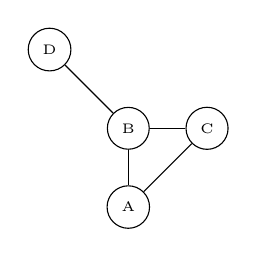
\begin{tikzpicture}
    \node[shape=circle,draw=black] (v1) at (0,0) {\tiny A};
    \node[shape=circle,draw=black] (v2) at (0,1) {\tiny B};
    \node[shape=circle,draw=black] (v3) at (1,1) {\tiny C};
    \node[shape=circle,draw=black] (v4) at (-1,2) {\tiny D};

    \draw (v1) -- (v2);
    \draw (v1) -- (v3);
    \draw (v2) -- (v4);
    \draw (v2) -- (v3);

  \end{tikzpicture}
\end{center}
In this picture, each circle corresponds to a vertice and each line corresponds
to a an edge; i.e. this diagram describes the graph
\[
  (\underbrace{\set{A, B, C, D}}_V,
  \underbrace{\set{(A, B), (A, C), (B, C), (B, D)}}_E).
\]
Note that we already use the convention that in an unoriented graph the pairs
are unordered and we have not listed $(B, A)$, $(C, A)$ etc.

To talk about graphs we need to fix the vocubulary.
An edge is said to \emph{connect} its endpoints; two vertices that are
connected by an edge are called \emph{adjacent}; and a vertex that is an
endpoint of a loop is said to be \emph{adjacent to itself}. An edge is said to
be \emph{incident} on each of its endpoints, and two edges incident
on the same end point are called \emph{adjacent}. A vertex on which no edges
are incident is called \emph{isolated}.

One of the most important examples of graphs are complete graphs defined as
follows.
\begin{definition}
  Let $n$ be a natural number. A complete graph on $n$ vertices, denoted
  $K_n$,\footnote[][-2cm]{%
    Some sources claim that the letter K in this notation stands for the German
    word komplett, but the German name for a complete graph, vollst\"{a}ndiger
    Graph, does not contain the letter K, and other sources state that the
    notation honors the contributions of Kazimierz Kuratowski to graph theory.
  } 
  is a simple graph with $in$ vertices and exactly one edge connecting
  each pair of distinct vertices.
\end{definition}
\nomenclature[G]{$K_n$}{denotes the complete graph on $n$ vertices}

\begin{exercise}
  Show that for all natural numbers $n$, the number of edges of $K_n$
  is $\frac{n(n - 1)}{2}$.
\end{exercise}

\section{Operations on Graphs}
Quite often in order to prove a theorem we need to modify a graph. The most
often operations are the following four. Let $G = (V, E)$ be a graph,
$F \subseteq E$ be a set of edges, $U \subseteq V$ be a set of edges,
$e \in E$ be an edge, and $v \in V$ be a vertex.
\begin{enumerate}
  \item $G[U]$ denotes the graph $(U, \set[e \in U^2]{e \in E})$,
    $G[U]$ is called the induced subgraph of $G$ on the vertices $U$;
    \nomenclature[G]{$G[U]$}{denotes the induced subgraph of $G$ on the vertices $U$
    (i.e. $(U, \set[e \in U^2]{e \in E})$)}
  \item $G[F]$ denotes the graph $(V, F)$, $G[F]$ is called the induced
    subgraph of $G$ on the edges $F$;
    \nomenclature[G]{$G[F]$}{denotes the induced subgraph of $G$ on the edges $F$
    (i.e. $(V, F)$)}
  \item $G - e$ denotes the graph $(V, E \setminus \set{e})$, i.e., the graph $G$
    without the edge $e$.
    \nomenclature[G]{$G - e$}{denotes the graph $(V, E \setminus \set{e})$}
  \item $G - v$ denotes the graph
    $(V \setminus \set{v}, E \cap (V \setminus \set{v})^2)$, i.e., the graph $G$
    without the vertex $v$.
    \nomenclature[G]{$G - v$}{denotes the graph
      $(V \setminus \set{v}, E \cap (V \setminus \set{v})^2)$}
\end{enumerate}

Note that we used the word ``subgraph'', in fact we can define formally the
meaning of this word.
\begin{definition}
  We say that a graph $H = (U, F)$ is a \emph{subgraph} of $G = (V, E)$ iff
  $U \subseteq V$ and $F \subseteq E$.
\end{definition}

\section{Degrees of Vertices}
The degree of a vertex is the number of endsegments of edges that ``stick out
of'' the vertex.
\begin{definition}
  Let $G = (V, E)$ be a graph, and $v$ be a vertex. Then
  $\deg_G(v) = |\set[{e \text{is connected to } v}]{e \in E}|$.
\end{definition}

\begin{exercise}
  Let $G = (V, E)$ be a graph and $v \in V$ be a vertex.
  What are the possible values of $\deg_G(v)$?
\end{exercise}

Note that Lemma~\ref{lemma:handshaking} shows that in any simple graph the
number of vertices with an odd degree is even.
The essence of the proof of this lemma is the following statement.
\begin{theorem}
  Let $G = (V, E)$ be a simple graph. Then $\sum_{v \in V} \deg_G(v) = 2|E|$.
\end{theorem}

\begin{chapterendexercises}
  \exercise Either draw a graph with the specified properties or explain why
    no such graph exists:
    \begin{enumerate}[nolistsep]
      \item simple graph with five vertices of degrees $1$, $2$, $3$, $3$,
        and $5$;
      \item simple graph with four vertices of degrees $1$, $2$, $3$, and $3$;
      \item simple graph with four vertices of degrees $1$, $1$, $1$, and $5$;
      \item simple graph with four vertices of degrees $1$, $2$, $3$, and $4$;
      \item simple graph with four vertices of degrees $1$, $2$, $3$, and $5$.
    \end{enumerate}
  \exercise In a group of $25$ people, is it possible for each to shake hands
    with exactly $3$ other people?
  \exercise Suppose that $G$ is a graph with $v$ vertices and $e$ edges and
    that the degree of each vertex is at least $d_\mathrm{min}$ and at most
    $d_\mathrm{max}$. Show that
    \[
      \frac{1}{2} v d_\mathrm{min} \le e \le \frac{1}{2} v d_\mathrm{max}.
    \]
\end{chapterendexercises}
